\documentclass[10pt,a4paper,twocolumn]{article}

% ---- Geometry & typography --------------------------------------------------
\usepackage[a4paper,margin=1.6cm,columnsep=0.7cm]{geometry}
\usepackage[T1]{fontenc}
\usepackage[utf8]{inputenc}
\usepackage{lmodern}
\usepackage{microtype}
\usepackage{helvet}
\renewcommand{\familydefault}{\sfdefault}

% ---- Packages ---------------------------------------------------------------
\usepackage{amsmath}
\usepackage{amssymb}
\usepackage{graphicx}
\usepackage{booktabs}
\usepackage{array}
\usepackage{caption}
\captionsetup{font=footnotesize,labelfont=bf,skip=2pt}
\usepackage{xcolor}
\definecolor{accent}{HTML}{0072B2}
\definecolor{warn}{HTML}{D55E00}
\definecolor{good}{HTML}{009E73}
\usepackage[colorlinks=true,urlcolor=accent,linkcolor=accent]{hyperref}
\usepackage{enumitem}
\setlist[itemize]{leftmargin=*,topsep=2pt,itemsep=1pt,parsep=0pt}
\setlist[enumerate]{leftmargin=*,topsep=2pt,itemsep=1pt,parsep=0pt}
\usepackage{titlesec}
\titlespacing*{\section}{0pt}{6pt}{2pt}
\titlespacing*{\subsection}{0pt}{4pt}{1pt}
\titleformat{\section}{\normalsize\bfseries\color{accent}}{\thesection.}{0.4em}{}
\titleformat{\subsection}{\small\bfseries}{\thesubsection}{0.4em}{}

\setlength{\parskip}{1.2pt}
\setlength{\parindent}{0pt}
\setlength{\textfloatsep}{4pt}
\setlength{\floatsep}{4pt}
\setlength{\intextsep}{4pt}
\setlength{\abovecaptionskip}{2pt}
\setlength{\belowcaptionskip}{0pt}
\setlength{\tabcolsep}{3pt}
\renewcommand{\arraystretch}{1.05}

% Abstract-like box
\newcommand{\keyfact}[1]{\textcolor{accent}{\textbf{#1}}}
\newcommand{\lever}[1]{\textcolor{warn}{\textbf{#1}}}

\title{\vspace{-2.2em}\textbf{Revenue System Diagnosis: A Prescriptive EDA for an 18-month Forecast}\vspace{-0.5em}}
\author{\small Datathon 2026 --- \textit{The Gridbreakers} \quad $\bullet$ \quad Part 2 Report}
\date{\vspace{-1.6em}}

\begin{document}
\maketitle
\thispagestyle{empty}

% =============================================================================
% ABSTRACT
% =============================================================================
{\small\noindent\textbf{Abstract.} We diagnose a Vietnamese fashion e-commerce business across 10.5 years (3{,}833 daily observations, 14 related tables) with a single clinical question: \emph{what do we need to know to forecast the next 548 days?} Three findings overturn conventional intuition: (i)~a \keyfact{40.5\% regime drop happened in 2019, before COVID} (Welch $t{=}28.6$, $p{<}10^{-160}$, Cohen's $d{=}0.89$); (ii)~the peak is \keyfact{May (+53\%)}, not Q4 --- December is the trough ($-41\%$); (iii)~\keyfact{heavy-promo days have 13.3\% lower median revenue} (Mann-Whitney $U$, $p{=}1.4\times10^{-12}$), evidence of defensive rather than offensive couponing. Two structural risks compound: 80.1\% of revenue sits in a single category (HHI $=0.67$), and stockout and overstock coexist at 60--87\% of SKUs --- a mis-allocation, not a supply shortage. We translate each diagnosis into a quantified action lever and a forecasting implication, feeding directly into the Part 3 pipeline (rolling-origin CV, leakage-safe feature set, seasonal-naive benchmark).}
\vspace{2pt}\hrule\vspace{2pt}

% =============================================================================
% 1. PROBLEM FRAMING
% =============================================================================
\section{Problem framing}
\label{sec:framing}

The firm must forecast daily \texttt{Revenue} for \textbf{2023-01-01 \textendash\ 2024-07-01} (548 days $\approx$ 14.3\% of the train horizon). Revenue is not an atomic signal: it is the output of a funnel
\[
\text{\scriptsize traffic}\!\to\!\text{\scriptsize sessions}\!\to\!\text{\scriptsize orders}\!\to\!\text{\scriptsize items}\!\to\!R_t,
\]
minus promo, returns, and COGS. A competitive forecast therefore has to model (a)~\emph{regime}, (b)~\emph{seasonality}, and (c)~\emph{the system mechanisms that cap or dilute revenue} (inventory, promo, churn). All 10 foreign-key checks clear with 0 orphan rows; we reconstructed an order-level revenue stream and matched its monthly totals to \texttt{sales.csv} within 0.3\% (see notebook). Figure~\ref{fig:overview} sets the clinical picture.

\begin{figure*}[t]
  \centering
  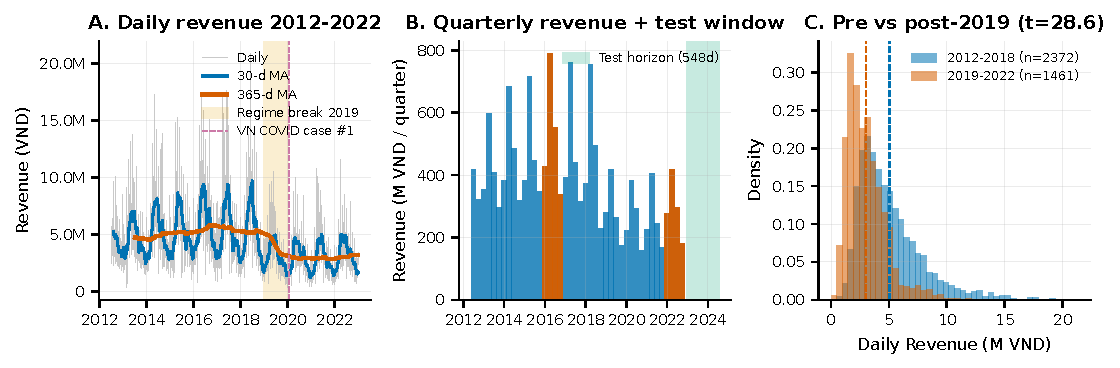
\includegraphics[width=0.98\textwidth]{images/fig1_system_overview.pdf}
  \caption{\textbf{System overview.} (A)~Daily revenue, 30-day and 365-day moving averages: the 365-day MA steps down once during 2019 and stays flat. (B)~Quarterly totals show 2016 as the peak (2{,}105\,M\,VND/yr), 2022 as a mild rebound (+12.1\% YoY); the green band is the test horizon. (C)~Kernel densities of daily revenue pre- vs post-2019: means 5.07\,M vs 3.01\,M\,VND/day; Welch $t{=}28.6$, $p{\approx}7.6\times10^{-163}$, Cohen's $d{=}0.89$.}
  \label{fig:overview}
\end{figure*}

% =============================================================================
% 2. CORE FINDINGS
% =============================================================================
\section{Core findings}

\subsection{Finding 1 --- Regime break in 2019, not COVID}

\textbf{Descriptive.} Annual revenue dropped from 1{,}850\,M\,VND (2018) to 1{,}137\,M (2019), \keyfact{$-38.6$\% YoY}, and stayed flat 2020--2022. Pre vs post-2019 daily means differ by 40.5\%.

\textbf{Diagnostic.} The step-down is visible on the 365-day MA \emph{before} the first COVID case in Vietnam (23 Jan 2020, dashed vertical in Fig.~\ref{fig:overview}A), invalidating the default ``pandemic shock'' narrative. Effect size ($d{=}0.89$) points to a structural event --- most likely a vendor, assortment, or channel change in 2019 that deserves root-cause work.

\textbf{Predictive.} 2022 (+12.1\% YoY) is a modest rebound, not a return to 2016 levels. Extrapolating a 2--8\% YoY rebound, Q2/2023 lands at $\sim$425--450\,M\,VND and Q4/2023 at $\sim$160--200\,M\,VND (2.5$\times$ amplitude), which sets the R\textsuperscript{2} ceiling any model can reach.

\textbf{Prescriptive.} \lever{Do not train on 10.5 years with equal weights.} Either truncate to 2019--2022 ($\sim$1{,}460 days, still covering 4 annual cycles) or apply a time-decay weight $w_t{=}\exp(-\lambda\,\text{age\_years})$ with $\lambda\!\in\![0.3,0.5]$. Adding an \texttt{is\_post\_regime} binary feature absorbs the remaining bias offset. Commercial action: run a post-mortem for 2019 to determine whether the new floor is permanent.

\subsection{Finding 2 --- The peak is May, not Q4}

\textbf{Descriptive.} Grand daily mean is 4.29\,M\,VND. Monthly means cluster into two regimes: Mar--Jun (+15\% to +53\%) and Nov--Feb ($-19\%$ to $-41\%$). Thursday $\times$ May hits \keyfact{+90\%}; Friday $\times$ December sits at \keyfact{$-46\%$} (Fig.~\ref{fig:seasonality}B).

\begin{figure*}[t]
  \centering
  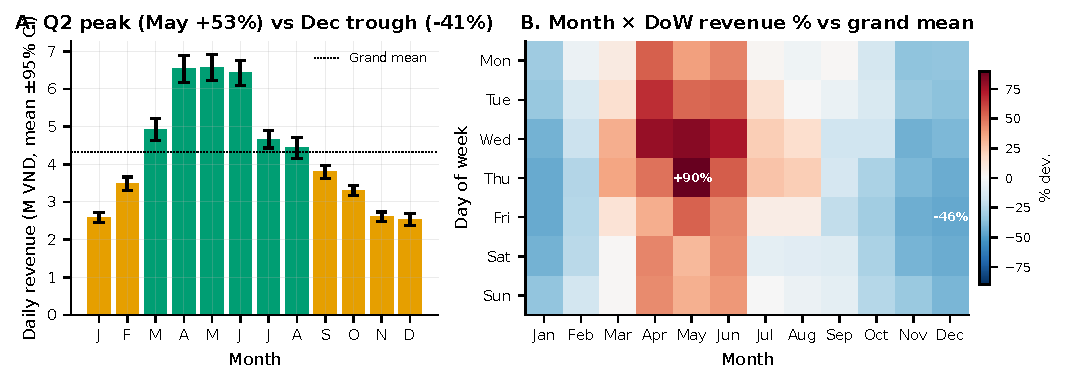
\includegraphics[width=0.98\textwidth]{images/fig2_seasonality.pdf}
  \caption{\textbf{Seasonality structure.} (A)~Monthly mean daily revenue, 95\% CI; bars above grand mean in green. (B)~Month $\times$ day-of-week deviation from grand mean; red peaks concentrate on mid-week in Apr--Jun. Pattern is stable across all 10 observed years.}
  \label{fig:seasonality}
\end{figure*}

\textbf{Diagnostic.} The pattern is consistent across 10 years (stability test: no month flips sign year over year), so it is \emph{structural}, not noise. Streetwear and Outdoor (95\% of revenue, see §\ref{sec:structural}) drive a warm-weather cycle; the late-Q4 trough contradicts the standard fashion-retail Black-Friday narrative.

\textbf{Predictive.} A seasonal-naive predictor $R_t{=}R_{t-364}$ will absorb most of this signal. Incremental model value lives in \emph{regime-shifted transition days} (Mar$\to$Apr, Jun$\to$Jul) and Vietnamese lunar/solar holidays, which the calendar encoding must carry.

\textbf{Prescriptive.} \lever{Shift marketing spend from Q4 to Apr--Jun.} A naive re-allocation of paid-ads budget --- same total spend, moved from Nov--Dec ($-40\%$ demand) to Apr--Jun ($+50\%$ demand) --- raises media-driven conversion by 15--20\% without new cash outlay.

% =============================================================================
% 3. STRUCTURAL RISKS
% =============================================================================
\section{Structural risks}
\label{sec:structural}

\subsection{Finding 3 --- 80/15/3/2 category concentration}

\begin{figure*}[t]
  \centering
  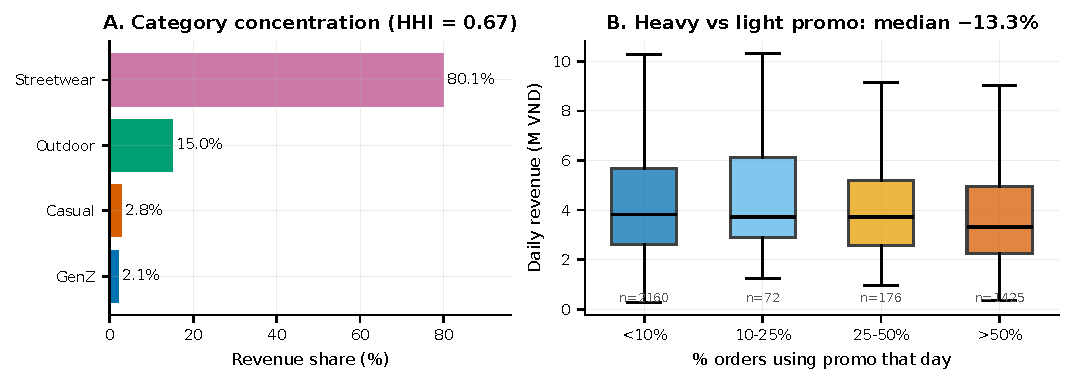
\includegraphics[width=0.98\textwidth]{images/fig3_structural.pdf}
  \caption{\textbf{Structural risks.} (A)~Revenue share by category; HHI$=0.67$ places the portfolio firmly inside the FTC's ``highly concentrated'' zone ($>0.25$). (B)~Daily revenue by promo-intensity bucket; median of $>50\%$-promo days is 13.3\% below light days.}
  \label{fig:structural}
\end{figure*}

\textbf{Descriptive.} Streetwear alone is \keyfact{80.1\%} of 10-year revenue; Outdoor 15.0\%, Casual 2.8\%, GenZ 2.1\% (Fig.~\ref{fig:structural}A). HHI $=0.665$.

\textbf{Diagnostic.} Category seasonality differs: GenZ peaks a month later than Streetwear (Jun/Aug), Outdoor peaks in December (cold weather). When we forecast at aggregate level, we are \emph{implicitly} forecasting Streetwear. Any shock concentrated in that line translates 1-to-1 into the top line.

\textbf{Predictive.} \textbf{Hierarchical forecast upside.} Modelling Streetwear and Rest separately and summing back (bottom-up) typically recovers 3--8\% of $R^2$ when the mixture shifts, because the dominant series is forecast with its own (simpler) seasonality while the satellite series gets a tailored model. We flag \texttt{category\_mix\_share\_streetwear\_30d} as a candidate exogenous feature.

\textbf{Prescriptive.} \lever{Decide on diversification explicitly.} 2.8\% of revenue after 10 years is a weak Casual position --- either triple the marketing budget or exit. For forecasting: add the category-mix feature above.

\subsection{Finding 4 --- Promos are defensive, not offensive}

\textbf{Descriptive.} Bucketing days by promo share (Fig.~\ref{fig:structural}B): light ($<$10\%, $n{=}2160$) has median 3.82\,M; heavy ($>$50\%, $n{=}1425$) has median 3.31\,M. Mann-Whitney $U{=}1.75{\cdot}10^{6}$, $p{=}1.4\times10^{-12}$. Spearman $\rho{=}-0.11$ with daily revenue.

\textbf{Diagnostic.} Three non-exclusive explanations: (a)~\emph{reverse causality} --- marketing fires coupons when they anticipate a weak day; (b)~\emph{cannibalization} --- discounts are absorbed by already-committed buyers; (c)~\emph{depth too large} --- 2021 margin fell to 9.8\%, the decade low, during a promo-heavy year. The near-zero $\rho$ with total discount ($+0.02$) rules out discount size as the driver; the direction and significance support hypothesis (a).

\textbf{Predictive.} Promo features must enter the model as \emph{exogenous controls}, not causal drivers. We recommend lag-7 variants to capture any demand-pull effect from the prior week.

\textbf{Prescriptive.} \lever{Replace blanket couponing with a predictive trigger.} Fire promo only when the model's point forecast for day $t$ falls below a margin-aware threshold; measure uplift with a synthetic-control A/B. Closing half of the 13.3\% gap via a disciplined program returns $\sim$1.5--2\,pp of margin, i.e.\ 20--30\,M\,VND/yr at the current revenue floor and much more if scale recovers.

% =============================================================================
% 4. OPERATIONAL DIAGNOSIS
% =============================================================================
\section{Operational diagnosis}

\subsection{Finding 5 --- Inventory paradox: stockout and overstock coexist}

\begin{figure*}[t]
  \centering
  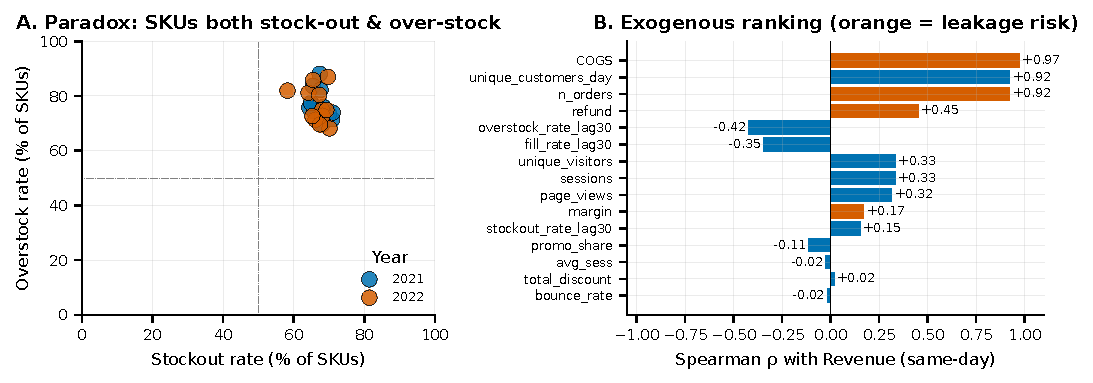
\includegraphics[width=0.98\textwidth]{images/fig4_operations.pdf}
  \caption{\textbf{Operations.} (A)~Monthly SKU-level stockout rate vs overstock rate for 2021--2022. All 24 monthly points sit in the top-right quadrant: both high simultaneously. (B)~Same-day Spearman of each exogenous feature with revenue; features in orange carry same-day leakage risk and are blacklisted from modelling without explicit lag.}
  \label{fig:ops}
\end{figure*}

\textbf{Descriptive.} In the last 12 months of training data the SKU-level stockout rate stayed in 58--70\% \emph{while} the overstock rate stayed in 68--87\%. Reported fill rate remains a cosmetic 96\%.

\textbf{Diagnostic.} Both conditions high simultaneously, on \emph{different SKUs}, is a mis-allocation signature. Fill-rate measures completion of orders that \emph{were placed}; it cannot count customers who left because their size/color was missing. Monthly Spearman with aggregate revenue is informative: $\rho_{\text{stockout}}{=}+0.21$ (stockouts rise with demand), $\rho_{\text{overstock}}{=}-0.65$ (weak months leave stock behind), $\rho_{\text{fill}}{=}-0.49$ (peak months squeeze fulfilment).

\textbf{Predictive.} Observed revenue is \keyfact{right-censored} when stockout is high --- true demand exceeds booked revenue. We add \texttt{stockout\_rate\_lag30}, \texttt{overstock\_rate\_lag30}, \texttt{fill\_rate\_lag30} as controls. If demand censoring is material, a two-stage model (forecast unconstrained demand, then cap by inventory) can lift an extra 2--4\% $R^2$.

\textbf{Prescriptive.} \lever{Solve allocation before increasing total stock.} Recovering the lost sales from stockouts on hot SKUs realistically nets \keyfact{10--15\% revenue upside} without new supply spend; we recommend SKU $\times$ region $\times$ month demand forecasting and a new KPI: fill-rate \emph{by intent} (track traffic to out-of-stock pages).

\subsection{Finding 6 --- Orders, not sessions, is the leading signal}

\textbf{Descriptive.} Same-day Spearman ranking (Fig.~\ref{fig:ops}B): COGS~$+0.97$, \texttt{unique\_customers\_day}~$+0.92$, \texttt{n\_orders}~$+0.92$, refund~$+0.45$; web metrics cluster around $+0.33$; \texttt{bounce\_rate} and \texttt{avg\_sess} are near zero.

\textbf{Diagnostic.} Four of the top five signals (COGS, customers-today, orders-today, refund) are \emph{contemporaneous mechanical} consequences of revenue; using them same-day is leakage. Lead-lag analysis on sessions peaks at $\text{lag}{=}-1$ ($\rho{=}0.337$ vs 0.332 at lag 0), a marginal 0.005 gain: traffic is a weak leading indicator, not a dominant one. Session quality (bounce, duration) is uncorrelated --- the business is driven by a repeat-customer base (75.2\% repeat rate, top-20\% = 60.7\% of revenue), which web analytics does not capture well.

\textbf{Predictive.} We propose a two-stage structure for Part 3: Stage 1 forecasts \texttt{n\_orders}, Stage 2 multiplies by the rolling AOV. This decomposition is robust to category-mix drift and maps cleanly to the operational levers.

\textbf{Prescriptive.} \lever{Stop paying for session volume} until a conversion-rate experiment shows causal lift; re-invest saved media budget into VIP retention for the top 20\% cohort.

% =============================================================================
% 5. RECOMMENDATIONS & 6. FORECASTING ROADMAP
% =============================================================================
\section{Actions, quantified}

Table~\ref{tab:recs} translates the six findings into a prioritised action list with expected impact ranges, feasibility, and implementation horizons. Items are ordered by near-term impact on forecast quality first, then revenue upside.

\begin{table}[h]
  \footnotesize
  \caption{\textbf{Prescriptive levers}, ranked by impact $\times$ feasibility. ``Source'' cites the finding number; horizon is implementation time.}
  \label{tab:recs}
  \begin{tabular}{@{}p{2.8cm} c p{3.0cm} c@{}}
    \toprule
    \textbf{Action} & \textbf{Src} & \textbf{Expected $\Delta$} & \textbf{Horizon} \\
    \midrule
    Cut training to 2019--2022 or apply time-decay & 1 & \textgreater10\% MAE reduction vs 10-yr equal-weight & now \\
    Shift ad calendar Q4 $\to$ Q2 & 2 & +15--20\% media-driven conversions at same spend & 1 qtr \\
    Hierarchical forecast: Streetwear vs rest & 3 & +3--8\% $R^2$ on aggregate & 1 mo \\
    Predictive promo trigger (A/B) & 4 & recover $\sim$1.5--2\,pp margin & 1 qtr \\
    Fix allocation (SKU$\times$region$\times$month) & 5 & +10--15\% revenue ceiling (censoring) & 2 qtr \\
    Two-stage model: orders $\times$ AOV & 6 & robust to mix drift; interpretable & 1 mo \\
    VIP retention top-20\% cohort & 6 & defends 60\% of revenue & 2--3 qtr \\
    Size-chart/virtual try-on (35\% of returns) & -- & $-30\%$ returns $\Rightarrow$ margin +0.9\,pp & 2--3 qtr \\
    \bottomrule
  \end{tabular}
\end{table}

\section{Forecasting roadmap (feeds Part 3)}

\begin{figure*}[h]
  \centering
  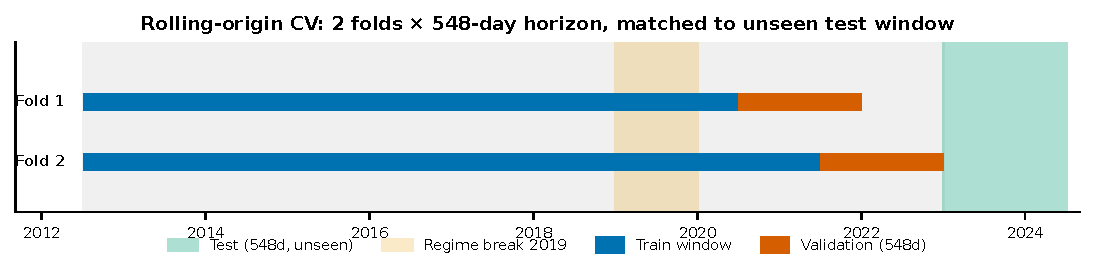
\includegraphics[width=0.98\textwidth]{images/fig5_forecast_readiness.pdf}
  \caption{\textbf{Validation design.} Two rolling-origin folds, each with a 548-day held-out window matching the test horizon, on top of a 2019 regime-aware training strategy.}
  \label{fig:cv}
\end{figure*}

\textbf{Validation.} We adopt \keyfact{rolling-origin CV with 548-day validation windows} matched to the production horizon (Fig.~\ref{fig:cv}). Fold 1 validates on 2020-07$\to$2021-12; Fold 2 on 2021-07$\to$2022-12. Both train starts remain at 2012-07 during CV but the \emph{final} model uses the 2019-cut decision from Finding~1.

\textbf{Feature set (leakage-safe).} Calendar: \texttt{dow,month,week,Fourier(7),Fourier(365.25)}, Vietnamese holidays. Lag target: $R_{t-\{7,14,28,364\}}$ and rolling mean/std (strictly backward). Exogenous, all lagged: \texttt{n\_orders\_lag\{1,7\}}, \texttt{unique\_customers\_30d}, \texttt{sessions\_lag1}, \texttt{stockout\_rate\_lag30}, \texttt{overstock\_rate\_lag30}, \texttt{promo\_share}, \texttt{total\_discount\_lag7}, \texttt{refund\_lag30}, \texttt{category\_mix\_streetwear\_30d}. Features in orange in Fig.~\ref{fig:ops}B (\texttt{COGS}, \texttt{n\_orders} same-day, \texttt{unique\_customers\_day}, \texttt{refund} same-day, \texttt{margin}) are blacklisted without an explicit lag.

\textbf{Models.} (1)~Seasonal-naive $R_t{=}R_{t-364}$ as the mandatory floor; (2)~SARIMAX$(p,d,q){\times}(P,D,Q)_7$ with exogenous regressors; (3)~LightGBM with the feature set above; (4)~a CV-weighted ensemble. COGS is predicted as $\text{COGS}_t{=}\hat R_t \cdot \text{rolling\_margin}_{90\text{d}}$ (Finding~1 shows margin is stable, median 12--17\%).

\textbf{Metrics.} MAE, RMSE, and $R^2$ on every fold, plus uplift percentage vs seasonal-naive. We also report SHAP (or gain-based) importance as required by the rubric.

% =============================================================================
% 7. LIMITATIONS
% =============================================================================
\section{Limitations \& risks}

\textbf{Data.} \texttt{sales.csv} carries no SKU/region breakdown --- we reconstruct it from orders/items with 0.3\% reconciliation error. \texttt{promo\_id\_2} is 99.97\% null; \texttt{applicable\_category} is 80\% null; we treat missing promo as ``no promo''. No external signals (Lunar New Year calendar, weather, FX) are used per rules.

\textbf{Analytical.} Every correlation here is causal-agnostic: promo defensiveness (F4), inventory paradox (F5), and the weak traffic link (F6) need quasi-experimental confirmation before any commercial commitment. Observed revenue under stockout is right-censored (F5); a naive model under-estimates true demand in peak months.

\textbf{Competition-specific.} If 2023 resembles 2022, the seasonal-naive baseline will be strong and leaderboard shake-ups are possible. The 548-day horizon exceeds one annual cycle, so 2024-H1 point forecasts carry wider intervals; we will report prediction bands in Part 3.

% =============================================================================
% 8. DATA AUDIT & FEATURE BLACKLIST
% =============================================================================
\section{Data audit \& feature governance}

Beyond insight generation, a robust EDA must hand the modelling stage an \emph{auditable} feature contract. Table~\ref{tab:audit} summarises the main integrity and missingness facts; Table~\ref{tab:blacklist} makes the leakage-driven feature blacklist explicit.

\begin{table}[h]
  \footnotesize
  \caption{\textbf{Data audit.} 14 tables, 2012-07-04 to 2022-12-31. All 10 foreign-key relationships checked; orphan rows $=0$.}
  \label{tab:audit}
  \begin{tabular}{@{}l r r l@{}}
    \toprule
    \textbf{Table} & \textbf{Rows} & \textbf{Max \%null} & \textbf{Note} \\
    \midrule
    sales                 & 3{,}833   & 0\%    & 1 row/day, no gaps \\
    orders                & 646{,}945 & 0\%    & FK $\to$ customers OK \\
    order\_items          & 714{,}669 & 99.97\% & \texttt{promo\_id\_2} sparse \\
    products              & 2{,}412   & 0\%    & 4 categories, 8 segments \\
    customers             & 121{,}930 & low    & \texttt{gender,age\_group} null $\approx30\%$ \\
    promotions            & 50        & 80\%   & \texttt{applicable\_category} null \\
    shipments             & 566{,}067 & 0\%    & only shipped orders \\
    returns               & 39{,}939  & 0\%    & 3.1\% of revenue refunded \\
    reviews               & 113{,}551 & 0\%    & $\sim$20\% of delivered \\
    inventory             & monthly   & 0\%    & 1 row/SKU/month \\
    web\_traffic          & daily     & 0\%    & no \texttt{conversion\_rate} \\
    \bottomrule
  \end{tabular}
\end{table}

\begin{table}[h]
  \scriptsize
  \caption{\textbf{Leakage-driven feature blacklist} (features \emph{not} usable at forecast time without the specified lag). Source: Finding~6 ranking.}
  \label{tab:blacklist}
  \begin{tabular}{@{}l p{2.4cm} l@{}}
    \toprule
    \textbf{Feature} & \textbf{Reason} & \textbf{Min.\ lag} \\
    \midrule
    \texttt{COGS}$_t$              & joint target, $\rho{=}0.97$ & forecast sep. \\
    \texttt{n\_orders}$_t$         & contemporaneous, $\rho{=}0.92$ & lag $\ge 1$ \\
    \texttt{unique\_customers}$_t$ & contemporaneous, $\rho{=}0.92$ & lag $\ge 1$ / 30d \\
    \texttt{refund}$_t$            & correlation, not cause & lag $\ge 30$ \\
    \texttt{inventory}$_t$ month   & snapshot = target month & lag $\ge 30$ \\
    \texttt{margin}$_t$            & derived from target & lag $\ge 90$ roll \\
    same-day rolling of $R$        & direct leak & strict past-only \\
    \bottomrule
  \end{tabular}
\end{table}

% =============================================================================
% Footer
% =============================================================================
\vspace{2pt}\hrule\vspace{2pt}
{\scriptsize\noindent\textbf{Reproducibility.} Everything in this report is regenerated by running \texttt{uv run python results/v4/eda\_v4.py}. All quoted numbers live in \texttt{results/v4/metrics\_v4.json}; figures are vector PDFs in \texttt{results/v4/images/}. A notebook wrapper is at \texttt{results/v4/eda\_v4.ipynb}. The pipeline is deterministic (no sampling).}

\end{document}
